\section{Mapserver}
MapServer adalah sebuah aplikasi freeware dan open source yang dapat menampilkan data spasial (peta) pada web. Aplikasi ini dikembangkan pertama kali oleh Universitas Minesotta, Amerika Serikat dalam projek ForNet yang merupakan sebuah projek untuk manajemen sumber daya alam yang disponsori NASA. kemudian dikembangkan projek TerraSIP sebagai manajemen data lahan. Karena sifatnya terbuka atau open source, pengembangan MapServer dilakukan oleh banyak negara.

Map Server bekerja beriringan dengan aplikasi web server. Web Server menerima request peta melalui MapServer, lalu MapServer mengenerate request terhadap peta lalu mengirimkannya ke web server seperti gambar dibawah ini.
\begin{figure}[ht]
	    \centerline{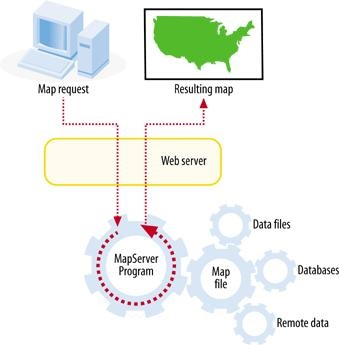
\includegraphics[width=0.50\textwidth]{figures/gambar5.JPG}}
	    \caption{Diagram operasi standar pada MapServer}
		\label{gambar5}
		\end{figure}
Fungsi utama dari MapServer yaitu untuk melakukan pembacaan data dari berbagai sumber dan menempatkannya kedalam layer-layer secara bersamaan yang kemudian menjadi file graphic.


\subsection{Pengertian MS4W}
MapServer for Windows (MS4W) adalah suatu packet software untuk mempermudah pengguna dalam menginstalasi MapServer pada platform OS Microsoft Windows. Tujuannya adalah untuk mempermudah semua user, terhindar dari segala bagian kecil yang rumit dalam mempersiapkan lingkungan kerja yang dibutuhkan oleh MapServer pada lingkungan Microsoft Windows. Software ini juga merupakan suatu cara yang bagus dalam memaketkan kemudian mendistribusikan aplikasi-aplikasi MapServer kepada pihak manapun.

\subsection{Cara Instalasi Mapserver}
\begin{enumerate}
\item
Download Mapserver atau disingkat MS4W di http://mapserver.org/download.html
\begin{figure}[ht]
	    \centerline{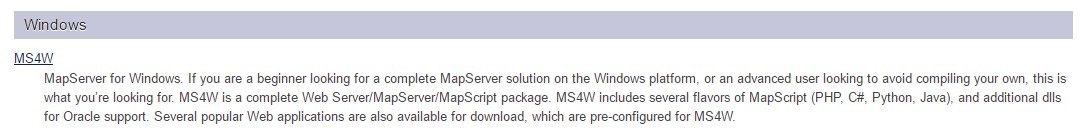
\includegraphics[width=0.50\textwidth]{figures/gambar1.JPG}}
	    \caption{Download MS4W}
		\label{gambar1}
		\end{figure}
\item
Setelah di download jalankan setupnya, disini saya menggunakan port 2000 karena port default 80 sudah dipakai oleh xampp
\begin{figure}[ht]
	    \centerline{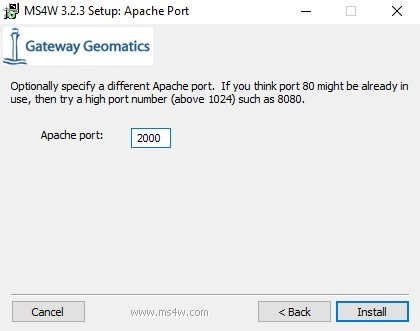
\includegraphics[width=0.50\textwidth]{figures/gambar2.JPG}}
	    \caption{Port 2000}
		\label{gambar2}
		\end{figure}
\item
Lalu tunggu instalasi sampai selesai
\begin{figure}[ht]
	    \centerline{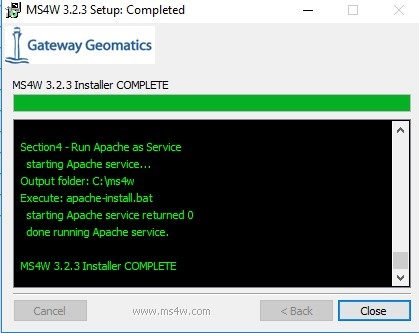
\includegraphics[width=0.50\textwidth]{figures/gambar3.JPG}}
	    \caption{Selesai}
		\label{gambar3}
		\end{figure}
\item
Setelah proses selesai silahkan buka browser favorit anda, kemudian ketikkan http://localhost:2000 di kotak isian URL.
\item
Jika anda melihat tampilan home MAPSERVER atau MS4W proses instalasi anda berhasil.
\begin{figure}[ht]
	    \centerline{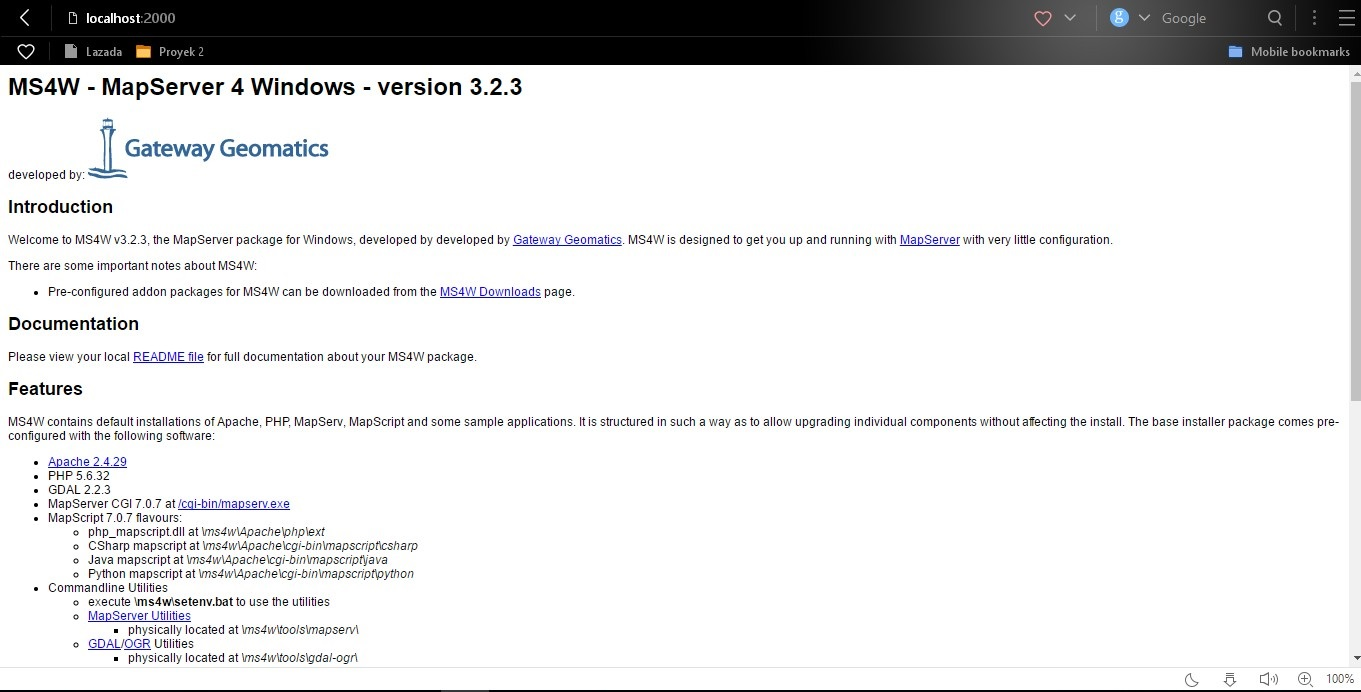
\includegraphics[width=0.50\textwidth]{figures/gambar4.JPG}}
	    \caption{Tampilan MS4W}
		\label{gambar4}
		\end{figure}
\end{enumerate}
